\chapter{Acceleration-Sensitive Interference}\label{chap:atom_int}
This chapter describes the work towards realising an atom interferometer and subsequently measuring accelerations.
\section{Chapter Outline}
\verysubsection{To-Do}
\begin{itemize}
    \item Raman spectrum, identifying each transition
    \item Characterisation of velocity-selective pulse and each interferometer pulse using Rabi oscillations.
    \item Making a three-pulse atom interferometer
    \item Improving acceleration sensitivity and correlating vibrations using MEMS
\end{itemize}
\section{Raman Optical System}\label{sec:setup_ramanoptics}

When designing an optical system for the light used in an atom interferometer, it is worth paying attention to both the spatial extent and beam waist of the collimated beam. These requirements are particularly important in this experiment, where acceleration due to gravity is perpendicular to the Raman beam axis and causes significant transverse motion of the atoms. Firstly, the optical system must be designed to make sure that the atoms are illuminated by each interferometer pulse. In addition to this, a more subtle requirement on the fringe contrast constrains the beam waist size. The gradient of intensity across the atom cloud must be small so that each atom is driven by (approximately) the same Rabi frequency. Otherwise, this variation in the Rabi frequency will dephase the atoms, which reduces the interferometer fringe contrast. 
For these reasons, it is beneficial to use a collimated laser beam which has a spatial extent much greater than the transverse distance travelled by the atoms and with a \(1/e^2\) radius much larger than the width of the atom cloud.

\subsection{Fringe Contrast Dependence}
The effects of a gradient of intensity on the fringe contrast can be shown by considering an ensemble of atoms that are spatially distributed by a Gaussian distribution. Neglecting the effect of the ensemble's velocity distribution on the Raman detuning and for fixed pulse times, the pulse area \(\Omega \tau\) varies only as a function of the radial displacement from the optic axis. The total fringe contrast can be determined by a convolution of the contrast for a single atom with the atomic density
\begin{equation}
    \mathcal{C} = \int \frac{1}{\sqrt{2\pi}\sigma_c}e^{-r^2/(2\sigma_c^2)} f_{\pi/2-\pi-\pi/2}\left(\Omega(r-r_1),\Omega_(r-r_2),\Omega(r-r_3)\right) \;\mathrm{d}r
    \label{eq:cloud_contrast}
\end{equation}
where \(\sigma_c\) is the radial width of the atom cloud, \(f_{\pi/2-\pi-\pi/2}\) is the fringe contrast as previously described in \EquationRef{eq:fringe_contrast} and \(r_i\) is the position of the ensemble's centre-of-mass at the \(i\)-th pulse. If the atom cloud is initially at the centre of the laser and falling under gravity, then these coordinates are \(\left(0, -\frac{1}{2}g T^2, -2 g T^2\right)\) respectively. Under the assumption that the two lasers which drive the Raman transition have the same waist size, the Rabi frequency, which is determined by the product of the electric fields (see~\EquationRef{eg:raman_rabi}), can be described by 
\begin{equation}
    \Omega(r) = \Omega_0 e^{-2 r^2/w^2}
\end{equation}
where \(\Omega_0\) is the Rabi frequency along the optic axis and \(w\) is the waist size -- the distance at which the electric field falls to \(1/e\) of its peak value. The fringe contrast as a function as beam waist for an atom cloud of width a width \(\sigma_c = \sivalue{5}{\milli\metre}\) and a time between interferometer pulses of \(T = \sivalue{25}{\milli\second}\) is plotted in \FigureRef{fig:raman_fringecontrast}. For small beam waists, the intensity gradient across the cloud significantly reduces the fringe contrast. In fact, a beam waist much greater than the width of the cloud is necessary to achieve a large contrast between the two interferometer states. Relaxing the assumptions made on the ensemble's velocity distribution to include its influence on the detuning and spatial distribution of the atoms during the interferometer would strengthen this argument.
\begin{figure}[h!]
    \centering
    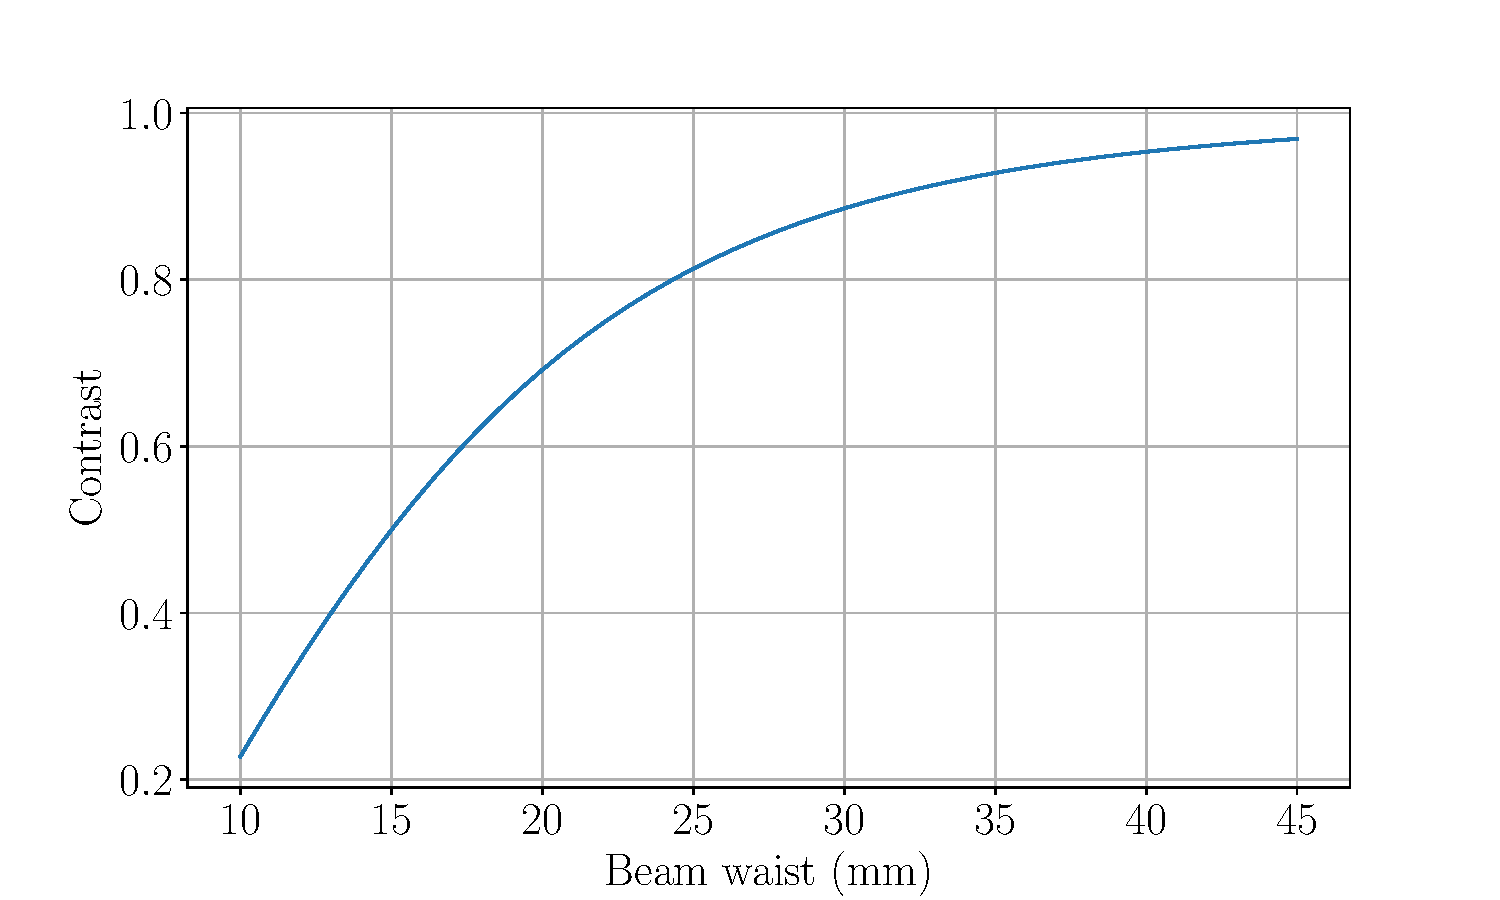
\includegraphics[width=0.5\textwidth]{fringeContrast.pdf}
    \caption[Simulated fringe contrast vs beam waist size]{Simulated fringe contrast as a function of waist size \(w\) for an atom cloud falling under gravity. This model assumes a Gaussian distributed atomic density with a width \(\sigma_c = \sivalue{5}{\milli\metre}\) and a time between interferometer pulses of \(T = \sivalue{25}{\milli\second}\). For smaller beam waists the subsequent interferometer pulses have a larger intensity gradient across the atom ensemble, which increases the dephasing of the two states and reduces the interferometer fringe contrast.}
    \label{fig:raman_fringecontrast}
\end{figure}

\subsection{Raman Beam Collimator}\label{subsec:setup_ramancollimator}
So far, it has been shown that a large beam waist is necessary to achieve a high fringe contrast when allowing for transverse motion of the atoms across the laser wavefront. Otherwise, if the fringe contrast was poor, this would limit the sensitivity of the interferometer to accelerations rather than other effects which are less rectifiable. Another optical effect which influences the sensitivity, and thus requires consideration, is distortions of the laser wavefront. In an ideal case, the superposition of the spherical wavefronts of the two lasers results in a planar wavefront for the effective field which drives the Raman transition. However, propagation through rough optical elements distort these wavefronts and introduce a spatially varying component of the Raman phase that is independent of acceleration. If the atom cloud's trajectory is parallel with the Raman axis, then this phase distortion is the same at each laser pulse and is therefore cancelled out. Of course, this does not occur when the cloud moves transverse to the Raman axis where this random phase has the effect of reducing the fringe contrast. 
\subsection{Retro-reflection Assembly}\label{subsec:setup_ramanmirror}
\subsubsection{In-Vacuum Alignment}
\subsection{The MEMS Accelerometer}\label{subsec:raman_mems}

\section{Driving Raman Transitions}
\subsection{Frequency and Phase Control}\label{subsec:msquared_comm}

\section{Atom Detection}
\subsection{Optical System}
\subsection{Measuring the Interferometer Phase}

\section{Individual Pulse Characterisation} \label{sec:atomint_rabiosc}
\subsection{Velocity-Selective Pulse}
\subsection{Interferometer Pulses}

\section{Three-Pulse Atom Interference} \label{sec:atomint_threepulse}

\section{Measuring Accelerations}\label{sec:atomint_accelerations}
\subsection{Vibration Sensitivity}